\documentclass[twoside]{book}

% Packages required by doxygen
\usepackage{fixltx2e}
\usepackage{calc}
\usepackage{doxygen}
\usepackage[export]{adjustbox} % also loads graphicx
\usepackage{graphicx}
\usepackage[utf8]{inputenc}
\usepackage{makeidx}
\usepackage{multicol}
\usepackage{multirow}
\PassOptionsToPackage{warn}{textcomp}
\usepackage{textcomp}
\usepackage[nointegrals]{wasysym}
\usepackage[table]{xcolor}

% Font selection
\usepackage[T1]{fontenc}
\usepackage[scaled=.90]{helvet}
\usepackage{courier}
\usepackage{amssymb}
\usepackage{sectsty}
\renewcommand{\familydefault}{\sfdefault}
\allsectionsfont{%
  \fontseries{bc}\selectfont%
  \color{darkgray}%
}
\renewcommand{\DoxyLabelFont}{%
  \fontseries{bc}\selectfont%
  \color{darkgray}%
}
\newcommand{\+}{\discretionary{\mbox{\scriptsize$\hookleftarrow$}}{}{}}

% Page & text layout
\usepackage{geometry}
\geometry{%
  a4paper,%
  top=2.5cm,%
  bottom=2.5cm,%
  left=2.5cm,%
  right=2.5cm%
}
\tolerance=750
\hfuzz=15pt
\hbadness=750
\setlength{\emergencystretch}{15pt}
\setlength{\parindent}{0cm}
\setlength{\parskip}{3ex plus 2ex minus 2ex}
\makeatletter
\renewcommand{\paragraph}{%
  \@startsection{paragraph}{4}{0ex}{-1.0ex}{1.0ex}{%
    \normalfont\normalsize\bfseries\SS@parafont%
  }%
}
\renewcommand{\subparagraph}{%
  \@startsection{subparagraph}{5}{0ex}{-1.0ex}{1.0ex}{%
    \normalfont\normalsize\bfseries\SS@subparafont%
  }%
}
\makeatother

% Headers & footers
\usepackage{fancyhdr}
\pagestyle{fancyplain}
\fancyhead[LE]{\fancyplain{}{\bfseries\thepage}}
\fancyhead[CE]{\fancyplain{}{}}
\fancyhead[RE]{\fancyplain{}{\bfseries\leftmark}}
\fancyhead[LO]{\fancyplain{}{\bfseries\rightmark}}
\fancyhead[CO]{\fancyplain{}{}}
\fancyhead[RO]{\fancyplain{}{\bfseries\thepage}}
\fancyfoot[LE]{\fancyplain{}{}}
\fancyfoot[CE]{\fancyplain{}{}}
\fancyfoot[RE]{\fancyplain{}{\bfseries\scriptsize Generated by Doxygen }}
\fancyfoot[LO]{\fancyplain{}{\bfseries\scriptsize Generated by Doxygen }}
\fancyfoot[CO]{\fancyplain{}{}}
\fancyfoot[RO]{\fancyplain{}{}}
\renewcommand{\footrulewidth}{0.4pt}
\renewcommand{\chaptermark}[1]{%
  \markboth{#1}{}%
}
\renewcommand{\sectionmark}[1]{%
  \markright{\thesection\ #1}%
}

% Indices & bibliography
\usepackage{natbib}
\usepackage[titles]{tocloft}
\setcounter{tocdepth}{3}
\setcounter{secnumdepth}{5}
\makeindex

% Hyperlinks (required, but should be loaded last)
\usepackage{ifpdf}
\ifpdf
  \usepackage[pdftex,pagebackref=true]{hyperref}
\else
  \usepackage[ps2pdf,pagebackref=true]{hyperref}
\fi
\hypersetup{%
  colorlinks=true,%
  linkcolor=blue,%
  citecolor=blue,%
  unicode%
}

% Custom commands
\newcommand{\clearemptydoublepage}{%
  \newpage{\pagestyle{empty}\cleardoublepage}%
}

\usepackage{caption}
\captionsetup{labelsep=space,justification=centering,font={bf},singlelinecheck=off,skip=4pt,position=top}

%===== C O N T E N T S =====

\begin{document}

% Titlepage & ToC
\hypersetup{pageanchor=false,
             bookmarksnumbered=true,
             pdfencoding=unicode
            }
\pagenumbering{alph}
\begin{titlepage}
\vspace*{7cm}
\begin{center}%
{\Large My Project }\\
\vspace*{1cm}
{\large Generated by Doxygen 1.8.13}\\
\end{center}
\end{titlepage}
\clearemptydoublepage
\pagenumbering{roman}
\tableofcontents
\clearemptydoublepage
\pagenumbering{arabic}
\hypersetup{pageanchor=true}

%--- Begin generated contents ---
\chapter{Main Page}
\label{index}\hypertarget{index}{}Class relations expressed via an inline dot graph\+: 
\begin{DoxyImageNoCaption}
  \mbox{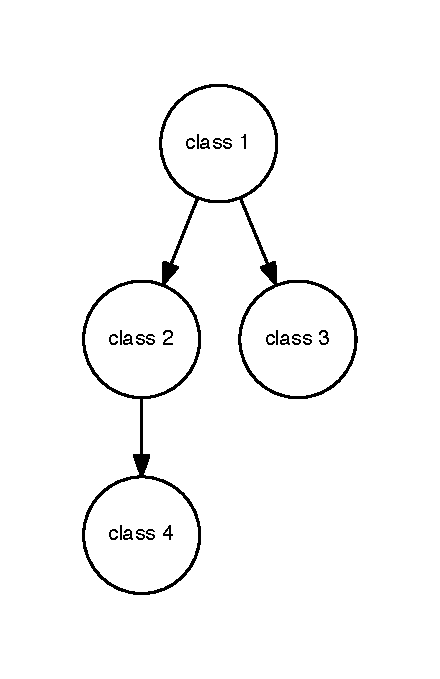
\includegraphics[width=\textwidth,height=\textheight/2,keepaspectratio=true]{dot_inline_dotgraph_1}}
\end{DoxyImageNoCaption}
 Note that the classes in the above graph are clickable (in the H\+T\+ML output). 
\chapter{Category}
\label{md_markdown_category}
\Hypertarget{md_markdown_category}

\begin{DoxyImageNoCaption}
  \mbox{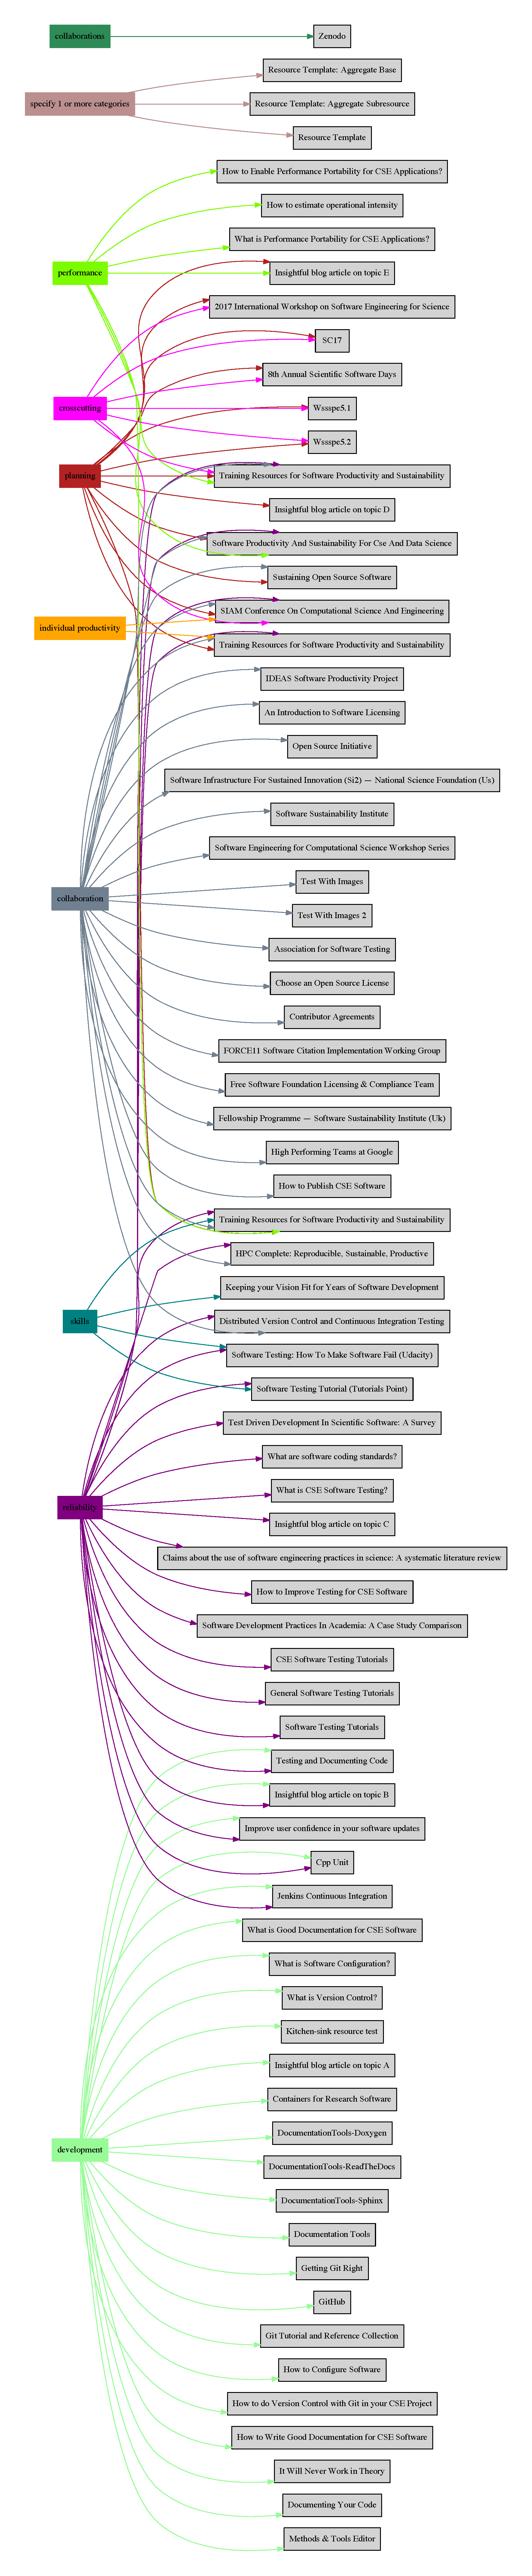
\includegraphics[width=\textwidth,height=\textheight/2,keepaspectratio=true]{dot_categories}}
\end{DoxyImageNoCaption}
 
\chapter{file1}
\label{md_markdown_file1}
\Hypertarget{md_markdown_file1}

\begin{DoxyCode}
#include <iostream>
using namespace std;

python
int main()\{
    cout << "Hello world";
\}
\end{DoxyCode}
 
\chapter{file2}
\label{md_markdown_file2}
\Hypertarget{md_markdown_file2}

\begin{DoxyCode}
#include <iostream>
using namespace std;


class file1;

int main()\{
    cout << "File2 depends on file1";
\}
\end{DoxyCode}
 
\chapter{file3}
\label{md_markdown_file3}
\Hypertarget{md_markdown_file3}

\begin{DoxyCode}
#include <iostream>
using namespace std;


class file1;

int main()\{
    cout << "File3 depends on file1";
\}
\end{DoxyCode}
 
\chapter{file4}
\label{md_markdown_file4}
\Hypertarget{md_markdown_file4}

\begin{DoxyCode}
#include <iostream>
using namespace std;


class file2;

int main()\{
    cout << "File4 depends on file2";
\}
\end{DoxyCode}
 
\chapter{This is header}
\label{md_markdown_intro1}
\Hypertarget{md_markdown_intro1}

\begin{DoxyImageNoCaption}
  \mbox{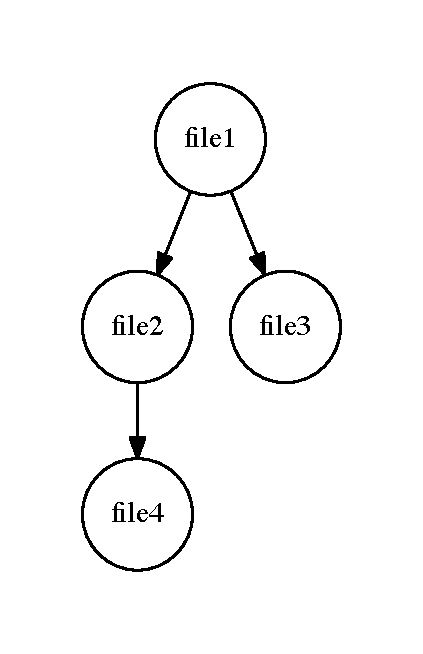
\includegraphics[width=\textwidth,height=\textheight/2,keepaspectratio=true]{dot_grap2}}
\end{DoxyImageNoCaption}
 
\chapter{Level}
\label{md_markdown_level}
\Hypertarget{md_markdown_level}

\begin{DoxyImageNoCaption}
  \mbox{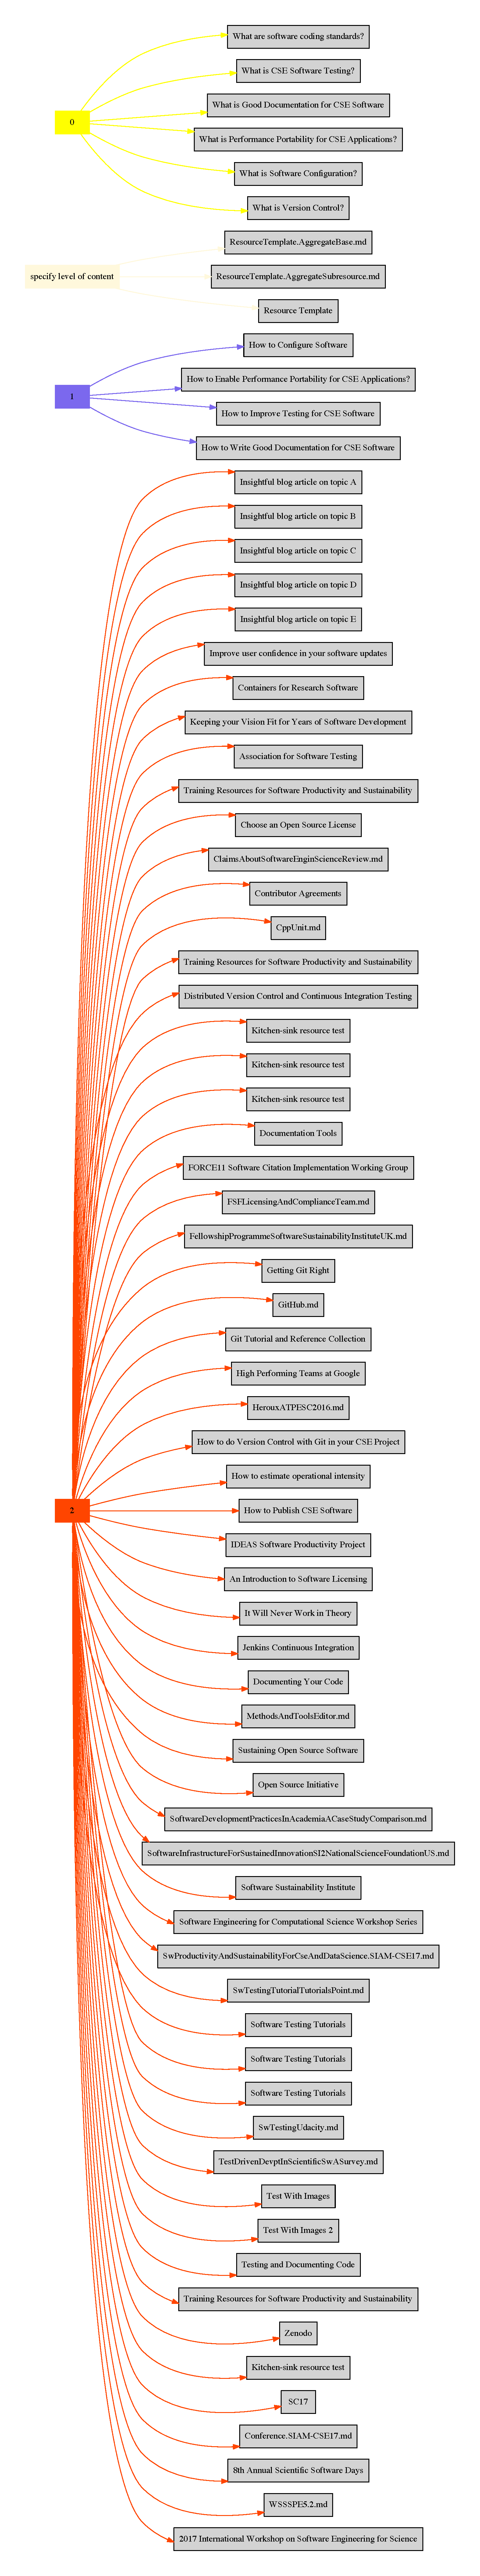
\includegraphics[width=\textwidth,height=\textheight/2,keepaspectratio=true]{dot_levels}}
\end{DoxyImageNoCaption}
 
\chapter{Tags}
\label{md_markdown_tags}
\Hypertarget{md_markdown_tags}

\begin{DoxyImageNoCaption}
  \mbox{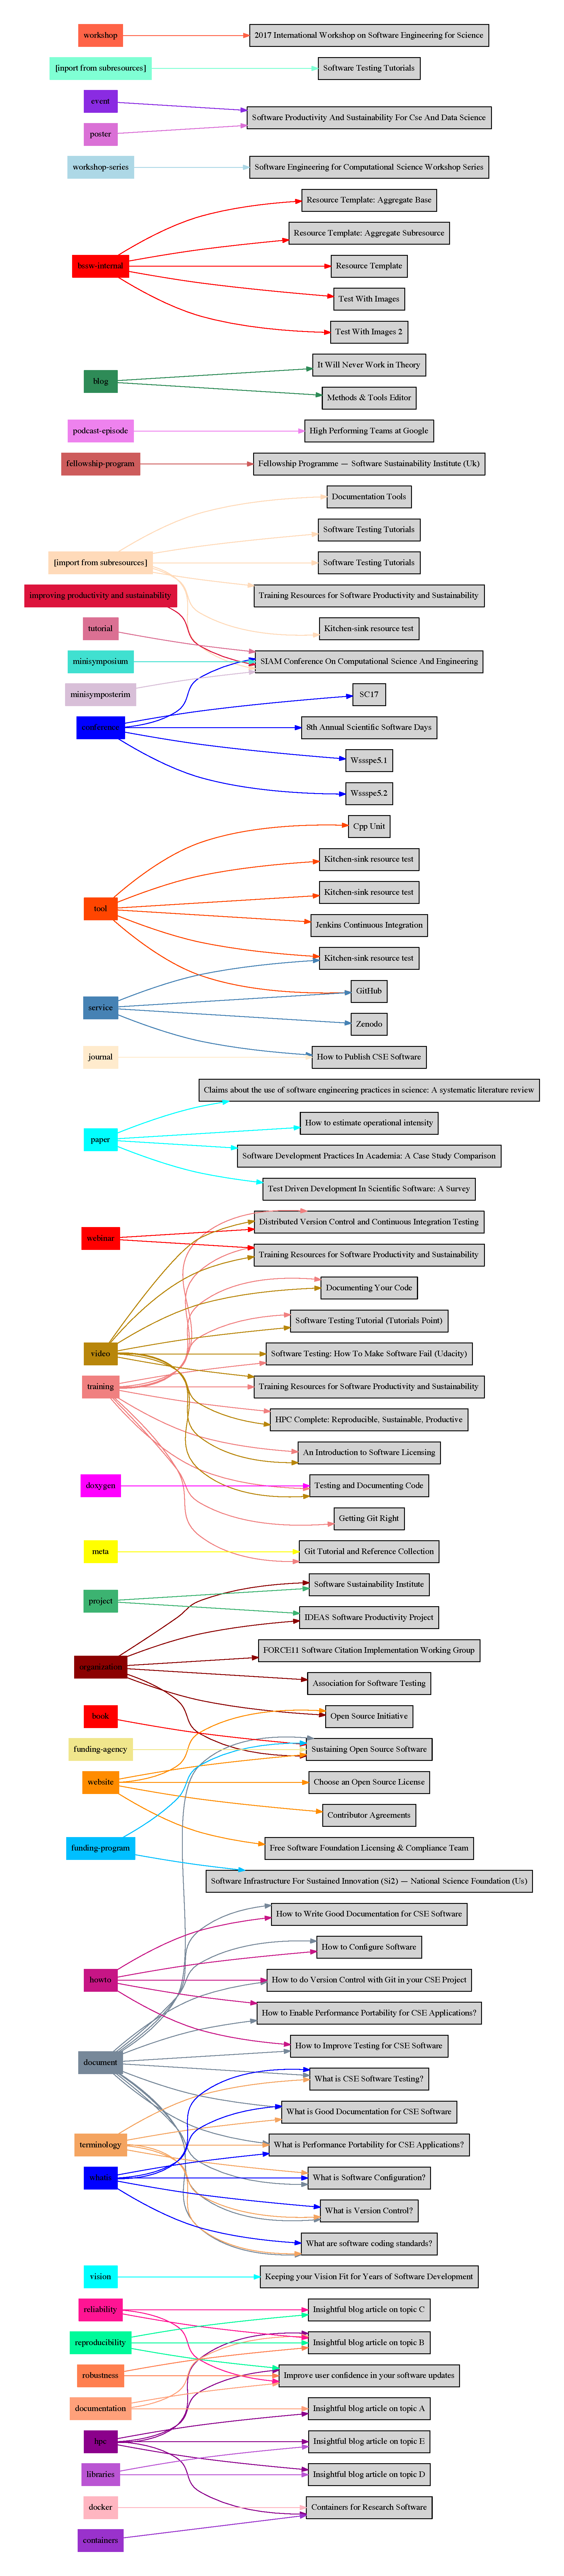
\includegraphics[width=\textwidth,height=\textheight/2,keepaspectratio=true]{dot_tags}}
\end{DoxyImageNoCaption}
 
\chapter{Topic}
\label{md_markdown_topic}
\Hypertarget{md_markdown_topic}

\begin{DoxyImageNoCaption}
  \mbox{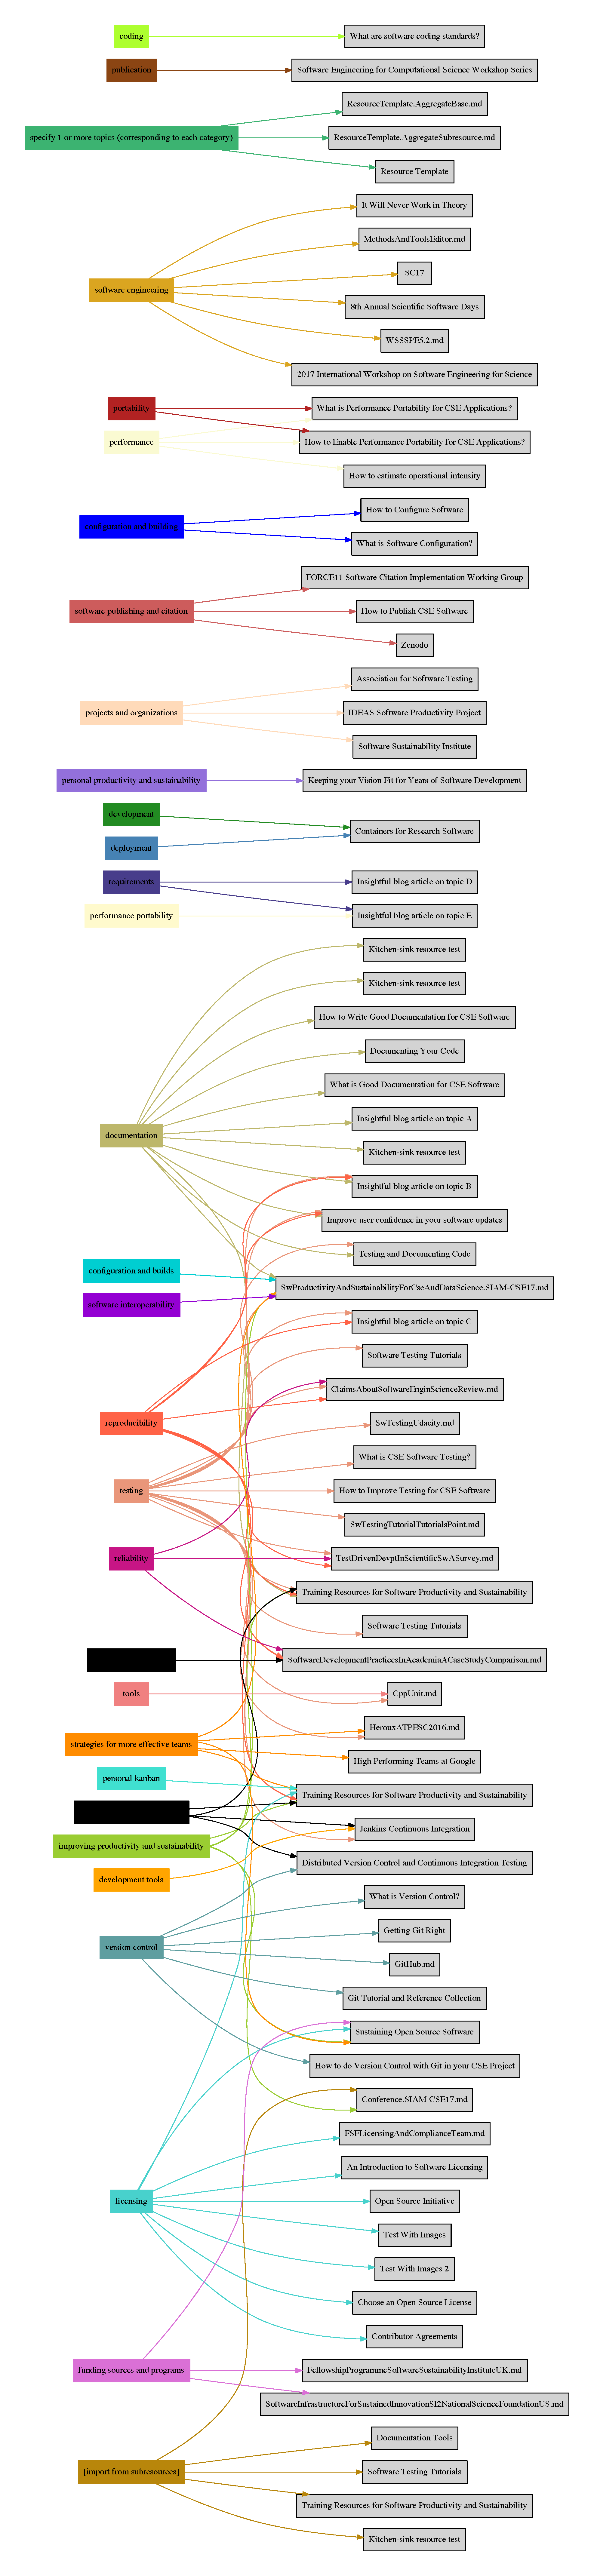
\includegraphics[width=\textwidth,height=\textheight/2,keepaspectratio=true]{dot_topics}}
\end{DoxyImageNoCaption}
 
\chapter{File Index}
\section{File List}
Here is a list of all files with brief descriptions\+:\begin{DoxyCompactList}
\item\contentsline{section}{markdown/\hyperlink{subfiles__generator_8py}{subfiles\+\_\+generator.\+py} }{\pageref{subfiles__generator_8py}}{}
\end{DoxyCompactList}

\chapter{File Documentation}
\hypertarget{category_8md}{}\section{markdown/category.md File Reference}
\label{category_8md}\index{markdown/category.\+md@{markdown/category.\+md}}

\hypertarget{file1_8md}{}\section{markdown/file1.md File Reference}
\label{file1_8md}\index{markdown/file1.\+md@{markdown/file1.\+md}}

\hypertarget{file2_8md}{}\section{markdown/file2.md File Reference}
\label{file2_8md}\index{markdown/file2.\+md@{markdown/file2.\+md}}

\hypertarget{file3_8md}{}\section{markdown/file3.md File Reference}
\label{file3_8md}\index{markdown/file3.\+md@{markdown/file3.\+md}}

\hypertarget{file4_8md}{}\section{markdown/file4.md File Reference}
\label{file4_8md}\index{markdown/file4.\+md@{markdown/file4.\+md}}

\hypertarget{intro_8java}{}\section{markdown/intro.java File Reference}
\label{intro_8java}\index{markdown/intro.\+java@{markdown/intro.\+java}}

\hypertarget{intro1_8md}{}\section{markdown/intro1.md File Reference}
\label{intro1_8md}\index{markdown/intro1.\+md@{markdown/intro1.\+md}}

\hypertarget{level_8md}{}\section{markdown/level.md File Reference}
\label{level_8md}\index{markdown/level.\+md@{markdown/level.\+md}}

\hypertarget{tags_8md}{}\section{markdown/tags.md File Reference}
\label{tags_8md}\index{markdown/tags.\+md@{markdown/tags.\+md}}

\hypertarget{topic_8md}{}\section{markdown/topic.md File Reference}
\label{topic_8md}\index{markdown/topic.\+md@{markdown/topic.\+md}}

%--- End generated contents ---

% Index
\backmatter
\newpage
\phantomsection
\clearemptydoublepage
\addcontentsline{toc}{chapter}{Index}
\printindex

\end{document}
